
\subsection{Cargas}
La carga es una unidad cuantizable, a partir de la carga del electrón \(e^{-}\),  siendo posible la carga una unidad de magnitud positiva o negativa. \par
Esta unidad afecta a nivel de la Fuerza Electrostática, el Campo Electrostático y sus magnitudes, y podemos considerar que todas las cargas poseen masa. \par
Además, dado un sistema, siempre \underline{la suma de todas las cargas va a ser cero}. De este enunciado podemos decir dos principios:


\begin{itemize}
        \item \underline{Principio de Conservación de la Carga}: La suma de todas las cargas del Universo vale cero, es decir, la carga total es \(cte\)
        \item \underline{Principio de Conservación local de la Carga}: La suma de todas las cargas en un sistema, es \(cte\) es decir, vale 0.
\end{itemize}
\subsection{Ley de Coulumb}
Esta es la ley fundamental que describe la interacción entre dos cargas puntuales en un medio, independientemente del tamaño del cuerpo. Consideramos la carga total del sistema, y no la unitaria por cada sección del cuerpo. \par
\hspace{4cm}
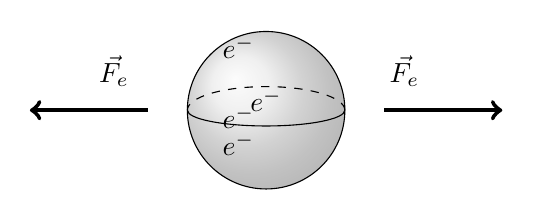
\begin{tikzpicture}
        \shade[ball color = gray!40, opacity = 0.4] (0,0) circle (1cm);
        \draw (0,0) circle (1cm);
        \draw (-1,0) arc (180:360:1 and  0.2);
        \draw[dashed] (1,0) arc (0:180:1 and 0.3);
        \node[left = 10, above = -20]{\(e^-\)};
        \node[left = 0, above = -4]{\(e^-\)};
        \node[left = 10, above = 15]{\(e^-\)};
        \node[left = 10, above = -10]{\(e^-\)};
        \node[right = 50, above = 5]{\(\vec{F_e}\)};
        \draw[->,ultra thick] (1.5,0)--(3,0);
        \node[right = -55, above = 5]{\(\vec{F_e}\)};
        \draw[->,ultra thick] (-1.5,0)--(-3,0);
\end{tikzpicture} \par
Cada cuerpo generará su propio campo y si consideramos las cargas puntuales, la fuerza entre ambas cargas será:
\[
        \boxed{\vec{F_{12}} = K \hspace{1mm}\frac{q_1q_2}{\left | \vec{r_2} - \vec{r_1} \right |^2}\hspace{2mm}\hat{r} = K \hspace{1mm}\frac{q_1q_2}{\left | \vec{r_2} - \vec{r_1} \right |^3}\hspace{2mm}(\vec{r_2} - \vec{r_1}) \hspace{3mm}N} \hspace{.25cm}
        \substack{\textnormal{\scriptsize{Siendo esta, el vector fuerza que ejerce la carga}} \\
                \textnormal{\(q_1\) sobre la carga \(q_2\).}}
\]
\[
        \boxed{\vec{F_{12}} = -\vec{F_{21}}} \hspace{.25cm}
        \substack{
                \textnormal{\scriptsize{Y evidentemente, el vector fuerza que ejerce la carga \(q_2\) sobre la carga \(q_1\) }}\\
                \textnormal{\scriptsize{es opuesta al vector fuerza que ejerce la carga \(q_1\) sobre la carga \(q_2\)}}
        }
\]
\newline
De esta forma podemos concluir con lo siguiente.
\begin{itemize}
        \item Las cargas de igual signo se repelen, mientras que las de signo diferente se atraen.
        \item Los vectores de posición son respecto a un punto de referencia.
\end{itemize}
\subsection{Campo Electrostático}
El campo es la manifestación de la perturbación en el espacio generado por una carga puntual:
\[
        \boxed{\vec{E} = \hspace{1mm}\frac{\vec{F_e}}{Q} \hspace{1mm}= \hspace{1mm} Kq\frac{\vec{r} -\vec{r`}}{\left | \vec{r} -\vec{r`} \right |^3} \hspace{3mm}V/m} \hspace{1cm}
        \substack{\textnormal{Siendo \(\vec{r`}\) el vector entre el punto de referencia y la carga y }
                \\
                \textnormal{\(\vec{r}\) es el vector entre el punto de estudio y el punto de referencia}
        }
\]
\\
Solo podemos calcular el campo cuando la carga \(q\) es muy pequeña, o lo que es lo mismo: \(\lim_{q \to 0} \vec{E} \approx 0\) \par
\vspace{1cm}
Sabiendo como se expresa el campo electrostático, nos interesaría conocer algunos casos puntuales dignos de consideración:
\begin{itemize}
        \item Dado un plano con dos cargas puntuales en el mismo eje de coordenadas, y queriendo calcular el campo en un punto cualquiera a una distancia equidistante respecto a las dos cargas es igual a:
              \begin{itemize}
                      \item \(\vec{E_x} = 2\left | \vec{E} \right | \cos{\alpha}\hspace{2mm} \hat{\imath}\)
                      \item \(\vec{E_y} = 2\left | \vec{E} \right | \sin{\alpha} \hspace{2mm} \hat{\jmath}\)
              \end{itemize}
        \item Las cargas actuan como sumideros.
        \item El campo generado por una carga eléctrica se emite de forma radial y constante, y su número indica su intensidad.
\end{itemize}
\subsection{Distribución de Cargas}
Hemos considerado un cuerpo cualquiera con carga, como una carga puntual que genera un \(\vec{E}\), ya que la carga se distribuía de forma continua. Sin embargo en la realidad no es así, y dependiendo del cuerpo que tengamos, su forma y tamaño afectarán al cálculo del campo. Para esto, deberemos de calcular sección por sección del cuerpo de estudio con el fin de obtener una aproximación del campo total. En esta parte veremos \underline{la distribución de cargas por unidad de longitud} que la denotaremos por:
\[ \boxed{\lambda = \frac{Q}{l}} \hspace{2cm} \textnormal{Siendo \(Q\) la carga y \(l\) la unidad de longitud}\]
Estudiaremos un caso muy particular, el campo generado por una barra metálica \\ infinítamente larga.\par
\vspace{0.5cm}
\hspace{4.5cm}
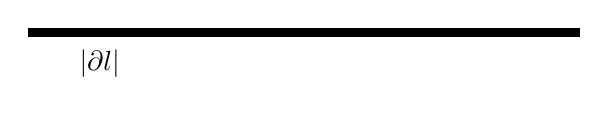
\begin{tikzpicture}
        \node[above = -10, right =15]{\(\left | \partial{l} \right |\)};
        \draw[draw=black, fill=black] (0,0) rectangle ++(7,0.1);
\end{tikzpicture}
\vspace{0.5cm}
\[
        \boxed{\vec{E}(P) \hspace{1mm} = \hspace{1mm}\frac{1}{4\pi\epsilon_o}\int^{b}_{a} \lambda \frac{\hat{r}}{r^2}\hspace{1mm} \mathrm{d}l \hspace{1mm} = K\lambda \int^{b}_{a}\frac{\vec{r}}{r^3} \mathrm{d}l\hspace{1mm} = K\lambda \int_{a}^{b} \frac{y}{h}\vec{\jmath} -\frac{x}{h} \vec{\imath} \hspace{2mm}\mathrm{d}l}
\]
Siendo \(h = \sqrt[]{x^2+y^2}\) y las incógnitas \(x\) e \(y\) como la distancia de un punto cualquiera en la barra para las coordenadas X e Y respectivamente.
\subsection{Ley de Gauss}
\hspace{10cm}
\begin{wrapfigure}{r}{3cm}
        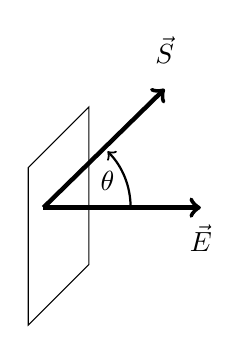
\begin{tikzpicture}[scale=2]
        \pgfmathsetmacro{\cubex}{2}
        \pgfmathsetmacro{\cubey}{1}
        \pgfmathsetmacro{\cubez}{1}
        \draw[] (0,0,0) -- ++(0,0,-\cubez) -- ++(0,-\cubey,0) -- ++(0,0,\cubez) -- cycle;
        \draw[->,ultra thick] (0,-.35,-0.25) --(1,-.35,-.25) node[above = -20]{\(\vec{E}\)};
        \draw[->,ultra thick] (0,-.35,-0.25) -- (30:1) node[above = 5]{\(\vec{S}\)};
        \draw[->,thick] (0.65,-.25) arc (0:45:0.5) node[above = -18]{\( \theta\)};
\end{tikzpicture}
\end{wrapfigure}
La ley de Gauss define el flujo de \(\vec{E}\) a través de una superficie cerrada.\par
Podemos considerar un caso general, donde dado un espacio cualquiera, con tamaño y forma indefinidos el flujo del campo eléctrico se denota por:
\[
        \phi =\lim_{\Delta S \to 0}\sum_{i=0}^{\infty}\vec{E_i}\hspace{1mm}\Delta S = \int_{S}\vec{E}\hspace{1mm}\mathrm{d} \vec{S} = \boxed{\oint_{S} \vec{E} \hspace{1mm}\mathrm{d} \vec{S} = \frac{Q_\textnormal{int}}{\epsilon_o}}
\]
Dada esta expresión podemos deducir que el flujo total es la suma, infinitesimal de cada una de las secciones sobre la que ejerce el campo eléctrico sobre la superficie, y que el flujo \(\phi\) es proporcional a la carga interna \(\Rightarrow \boxed{\phi \hspace{1mm} \alpha \hspace{1mm} q}\) \par
\vspace{1cm}
\hspace{-.5cm}
Por lo tanto podemos estudiar el valor del campo \(\vec{E}\) en casos de extrema simetría.
Para esto consideraremos una nueva magnitud \(\sigma\) que denota la \underline{distribución superficial de carga}. \(\boxed{\sigma = \frac{Q}{S}}\)
\par \vspace{.5cm} \hspace{-.5cm}No confundir la superficie del cuerpo de estudio con la superficie Gaussiana, esta es variable y depende de quien la estudie.
\subsubsection{Plano Infinito}
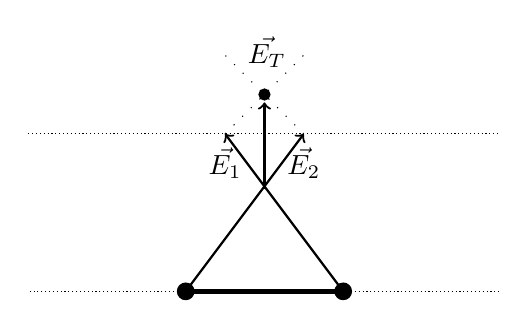
\begin{tikzpicture}
        \draw[densely dotted] (-2,2) -- (4,2);
        \draw[-,ultra thick] (0,0) -- (2,0);
        \draw[densely dotted] (2,0) -- (4,0);
        \draw[densely dotted] (0,0) -- (-2,0);
        \draw[->, thick] (2,0) -- (0.5,2) node[above = -20]{\(\vec{E_1}\)};
        \draw[->, thick] (0,0) -- (1.5,2) node[above = -20]{\(\vec{E_2}\)};
        \filldraw[color = black] (2,0) circle (3pt);
        \filldraw[color = black] (0,0) circle (3pt);
        \draw[loosely dotted] (0.5,2) -- (1.5,3) node[above = 1, left = 3]{\(\vec{E_T}\)};
        \draw[loosely dotted] (1.5,2) -- (0.5,3);
        \filldraw[color = black] (1,2.5) circle (2pt);
        \draw[->, thick] (1,1.3) -- (1,2.4);
\end{tikzpicture}\par
\hspace{-.5cm}Dado el diagrama propuesto, todos los puntos situados en el mismo plano, poseen la misma \\ \hspace{-.5cm} Distribución Superficial de Carga, y por ende todos los puntos poseen el mismo
\[\vec{E} = \vec{E_1} + \vec{E_2} = 2\vec{E}\]
\subsubsection{Cilindro en un plano infinito}
Si situaramos un cilindro en un plano infinitamente largo, observamos que el flujo corresponde a la suma del flujo que pasa por cada una de las tapas y la cubierta lateral del cilindo. De esta forma, debido a que la cubierta lateral es paralela al vector normal al campo, el flujo que pasa por ahí es nulo. Por ende:
\[
        \oint \vec{E}\hspace{1mm}\mathrm{d} \vec{S} = \oint_{SL}\vec{E}\hspace{1mm}\mathrm{d} \vec{S} +\oint_{S^+}\vec{E}\hspace{1mm}\mathrm{d} \vec{S}+\oint_{S^-}\vec{E}\hspace{1mm}\mathrm{d} \vec{S} =
        2 \oint_{S^+} \vec{E}\hspace{1mm}\mathrm{d} \vec{S} \Rightarrow \phi =2\left | \vec{E} \right |\left | \vec{S} \right | = 2ES
\]
\[
        2ES = \frac{Q_{\textnormal{int}}}{\epsilon_o} \Rightarrow E = \frac{\left | \sigma \right |}{2\epsilon_o} \Rightarrow \boxed{\vec{E} = \frac{\sigma}{2\epsilon_o}\hspace{1mm}\hat{n}}
\]
Posteriormente veremos que si el cuerpo está cargado y analizamos el campo \(\vec{E}\), este valdrá 0, y por ende su potencial es \(cte\) aunque no sepamos cuanto pueda valer.
\subsubsection{Esfera cargada}
Aplicando la Ley de Gauss y considerando \(R\) el radio de la superficie Gaussiana:
\[
        \oint \vec{E} \hspace{1mm} \mathrm{d}\vec{S} \Rightarrow \left | \vec{E} \right | 4\pi R^2 = \hspace{1mm} \frac{Q_{\textnormal{int}}}{\epsilon_o}
\]
\[
        \boxed{\vec{E}  = \hspace{1mm} \frac{Q_{\textnormal{int}}}{\epsilon_o4\pi R^2} \hspace{1mm}\hat{n} \hspace{1mm} = \frac{\sigma r^2}{\epsilon_o R^2} \hspace{1mm}\hat{n}}
\]
\vspace{3cm}
\subsection{Balance de Energías}
\begin{wrapfigure}{r}{5cm}
        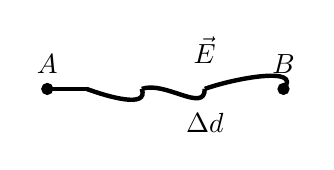
\begin{tikzpicture}
                \draw[-,ultra thick] (0,0) -- (0.5,0);
                \draw[-,ultra thick] (0.5,0) to[out=-20,in=-70] (1.2,0);
                \draw[-,ultra thick] (1.2,0) to[out=20,in=-90] (2,0) node[above =-20]{\(\Delta d\)} node[above =5]{\(\vec{E}\)};
                \draw[-,ultra thick] (2,0) to[out=20,in=50] (3,0);
                \filldraw[color = black] (0,0) circle (2pt) node[above =2]{\(A\)};
                \filldraw[color = black] (3,0) circle (2pt) node[above =2]{\(B\)};
        \end{tikzpicture}
\end{wrapfigure}
Debido a que la fuerza electrostática es una fuerza conservativa, no importa la ruta recorrida, sino las posiciones inicial y final para calcular el trabajo requerido para mover la carga de un punto A al B.\par
\vspace{0.5cm}
\hspace{-.725cm}
De esta forma podemos aplicar \underline{El Teorema de las Fuerzas Vivas} por lo que \(\boxed{W_{A \to B} = \Delta E_c = \frac{1}{2} m (V_B -V_A) \hspace{2mm}J}\)
\par
\vspace{0.5cm}
\hspace{-.6cm}
Por lo tanto el trabajo requerido para mover una carga de un punto A a otro B, es igual a \(\ \Rightarrow \boxed{W_{A \to B} =-\Delta E_p = -q \Delta V}\) \par
\vspace{0.5cm}
\[
        \textnormal{En funcion del signo} \rightarrow
        \begin{cases}
                \textnormal{Si \(W > 0\), \(q\) se mueve a favor del campo} \\
                \\
                \textnormal{Si \(W < 0\), \(q\) requiere de un \(W_{\textnormal{ext}}\) para moverse}
        \end{cases}
\]